\chapter{Use Cases}
\ChapterLabel{UseCases}
%\section{How to Use This Chapter}
%Describe goal-oriented interactions at the system boundary. Give every use case
%a stable ID, its own table, and at least one reciprocal requirement mapping.
%Include preconditions, trigger, main flow, alternate or exception flows, and
%postconditions. Maintain the canonical relationships among stories,
%requirements, use cases, and tests in \ChapterRef{Traceability}.

% \section[High-Level Use Case Diagram]{\hspace{0.5em}High-Level Use Case Diagram}
% Show the system boundary, primary actors, and major user goals before the
% detailed use-case tables. Replace the generic example with project-specific
% actors and use cases while preserving the stable use-case identifiers.

\begin{figure}[h]
\centering
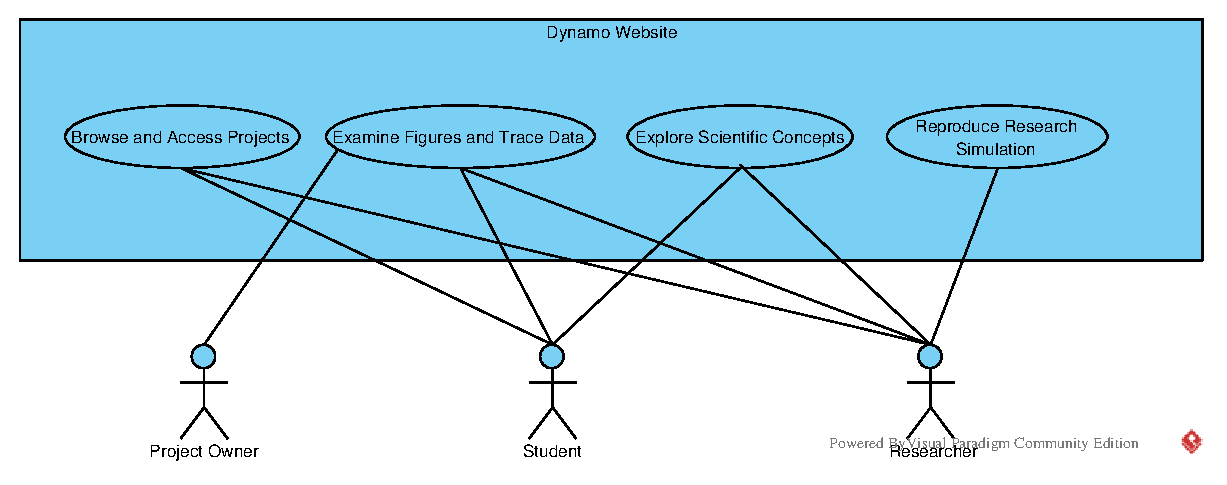
\includegraphics[width=0.88\textwidth]{eps/dsnUseCases/Dynamo_Diagram.eps}
\caption{Dynamo website use case diagram.\label{Figure:UseCaseDiagram}}
\end{figure}
\index{use case diagram}

\section{Browse and Access Research Projects}
\begin{tabularx}{\linewidth}{L{3.5cm}Y}
\toprule
\textbf{Identifier} & \UseCaseID{UC-001}\\
\textbf{Mapped requirements} & \RequirementRef{REQ-B-001}, \RequirementRef{REQ-Q-003}, \RequirementRef{REQ-Q-004}, \RequirementRef{REQ-Q-005}, \RequirementRef{REQ-S-004}, \RequirementRef{REQ-C-001}, \RequirementRef{REQ-C-003}\\
\textbf{Goal} & Allow users to find and access research papers, simulation code, datasets, and other research artifacts associated with a project.\\
\textbf{Primary actor} & Researcher, Student, or General Public\\
\textbf{Preconditions} & The website is accessible through a supported web browser and the requested research project exists on the platform.\\
\textbf{Trigger} & The user selects a research project from the website.\\
\textbf{Main flow} & The user browses or searches for a research project; the system displays the project overview and available research artifacts; the user selects an artifact; and the system retrieves and displays the selected artifact while distinguishing raw simulation output from processed or analyzed data.\\
\textbf{Alternate flow} & If the requested project or artifact does not exist, the system informs the user that no matching resource was found.\\
\textbf{Postconditions} & The selected research project or artifact has been displayed to the user without modifying the stored artifact.\\
\bottomrule
\end{tabularx}

\section{Explore Scientific Concepts}
\begin{tabularx}{\linewidth}{L{3.5cm}Y}
\toprule
\textbf{Identifier} & \UseCaseID{UC-002}\\
\textbf{Mapped requirements} & \RequirementRef{REQ-B-003}, \RequirementRef{REQ-F-001}, \RequirementRef{REQ-C-001}\\
\textbf{Goal} & Allow users to understand fundamental scientific concepts, variables, physical definitions, and units relevant to a research project.\\
\textbf{Primary actor} & Student, Researcher, or General Public\\
\textbf{Preconditions} & The research project contains documented scientific concepts or definitions.\\
\textbf{Trigger} & The user selects a scientific concept or definition associated with the research project.\\
\textbf{Main flow} & The user opens the project's concept documentation; the system displays an explanation of the selected concept; the system displays relevant scientific variables, physical definitions, and units; and the user reviews the information.\\
\textbf{Alternate flow} & If the selected concept does not have available documentation, the system informs the user that the concept has not yet been documented.\\
\textbf{Postconditions} & The user has access to the available explanation and definitions for the selected scientific concept.\\
\bottomrule
\end{tabularx}


\section{Examine Figures and Trace Supporting Data}
\begin{tabularx}{\linewidth}{L{3.5cm}Y}
\toprule
\textbf{Identifier} & \UseCaseID{UC-003}\\
\textbf{Mapped requirements} & \RequirementRef{REQ-B-004}, \RequirementRef{REQ-D-005}, \RequirementRef{REQ-C-001}\\
\textbf{Goal} & Allow users to understand key research figures and trace the figures back to the supporting data, analysis procedures, and simulation parameters.\\
\textbf{Primary actor} & Researcher, Third-Party Researcher, or General Public\\
\textbf{Preconditions} & The research project contains at least one documented figure and associated research data.\\
\textbf{Trigger} & The user selects a research figure.\\
\textbf{Main flow} & The user selects a figure; the system displays an explanation of the figure and its relationship to the research; the system displays the quantities and units represented by the figure; the system identifies the supporting data and processing or analysis procedure; and the system provides links to the relevant simulation parameters and source data.\\
\textbf{Alternate flow} & If supporting data or processing information is unavailable, the system displays the figure and available documentation while indicating which supporting information is unavailable.\\
\textbf{Postconditions} & The user can identify the relationship between the figure, supporting data, analysis procedure, and simulation parameters.\\
\bottomrule
\end{tabularx}


\section{Reproduce Results}
\begin{tabularx}{\linewidth}{L{3.5cm}Y}
\toprule
\textbf{Identifier} & \UseCaseID{UC-004}\\
\textbf{Mapped requirements} & \RequirementRef{REQ-B-005}, \RequirementRef{REQ-D-004}, \RequirementRef{REQ-D-005}, \RequirementRef{REQ-D-006}, \RequirementRef{REQ-C-001}\\
\textbf{Goal} & Provide a researcher with sufficient data, metadata, and procedures to reproduce a documented simulation and its associated analysis.\\
\textbf{Primary actor} & Researcher or Third-Party Researcher\\
\textbf{Preconditions} & The research project contains thorough instructions for reproducing results. \\
\textbf{Trigger} & The researcher selects a simulation and chooses to review its reproduction information.\\
\textbf{Main flow} & The researcher finds a project; a docker image and documentation are provided;\\
\textbf{Alternate flow} & If required reproduction information is missing, the system identifies the unavailable information and informs the researcher that the simulation cannot be fully reproduced from the available documentation.\\
\textbf{Postconditions} & The researcher has access to the available simulation inputs, metadata, data, and analysis procedures needed for reproduction.\\
\bottomrule
\end{tabularx}


\section{Manage Research Artifacts}
\begin{tabularx}{\linewidth}{L{3.5cm}Y}
\toprule
\textbf{Identifier} & \UseCaseID{UC-005}\\
\textbf{Mapped requirements} & \RequirementRef{REQ-F-003}, \RequirementRef{REQ-Q-001}, \RequirementRef{REQ-Q-002}, \RequirementRef{REQ-Q-003}, \RequirementRef{REQ-Q-005}, \RequirementRef{REQ-I-001}, \RequirementRef{REQ-I-002}, \RequirementRef{REQ-S-001}, \RequirementRef{REQ-S-002}, \RequirementRef{REQ-S-003}, \RequirementRef{REQ-S-005}, \RequirementRef{REQ-D-001}, \RequirementRef{REQ-D-004}, \RequirementRef{REQ-D-005}, \RequirementRef{REQ-D-006}, \RequirementRef{REQ-D-008}, \RequirementRef{REQ-C-001}, \RequirementRef{REQ-C-002}, \RequirementRef{REQ-C-003}\\
\textbf{Goal} & Allow authorized researchers to upload, edit, and manage research artifacts while maintaining version history and provenance.\\
\textbf{Primary actor} & Researcher or Project Owner\\
\textbf{Preconditions} & The researcher is authenticated and has appropriate permissions for the research project.\\
\textbf{Trigger} & The researcher chooses to upload or modify a research artifact.\\
\textbf{Main flow} & The researcher logs into their account; the system verifies the researcher's credentials; the researcher uploads or modifies an artifact such as code, data, images, videos, or a Docker image; the system stores the artifact without modifying its contents; the system records relevant metadata and provenance; and the system creates a timestamped version-history entry.\\
\textbf{Alternate flow} & If the researcher is not authenticated or does not have the required permissions, the system denies the requested modification. If the uploaded artifact is invalid or cannot be stored, the system reports the error and does not create the new version.\\
\textbf{Postconditions} & The authorized artifact has been stored or updated, and the modification is recorded in the artifact's version history and provenance information.\\
\bottomrule
\end{tabularx}


\section{Review Experiment History and Results}
\begin{tabularx}{\linewidth}{L{3.5cm}Y}
\toprule
\textbf{Identifier} & \UseCaseID{UC-007}\\
\textbf{Mapped requirements} & \RequirementRef{REQ-B-002}, \RequirementRef{REQ-F-002}, \RequirementRef{REQ-D-003}, \RequirementRef{REQ-D-004}, \RequirementRef{REQ-C-001}\\
\textbf{Goal} & Allow researchers to review experiments conducted for a project and examine the associated parameters and results.\\
\textbf{Primary actor} & Researcher or Third-Party Researcher\\
\textbf{Preconditions} & The research project contains a record of one or more experiments.\\
\textbf{Trigger} & The user opens the experiment history for a research project.\\
\textbf{Main flow} & The user selects a research project; the system displays the experiment log; the user selects an experiment; the system displays the experiment's initial conditions, input parameters, output dataset identifier, and relevant metadata; and the system allows results from different accretion disk scale heights to be compared.\\
\textbf{Alternate flow} & If an experiment does not contain complete result information, the system displays the available information and identifies missing data or metadata.\\
\textbf{Postconditions} & The user has reviewed the available experiment history and results, including the parameters associated with the selected experiment.\\
\bottomrule
\end{tabularx}


\section{Manage Collaboration and Access}
\begin{tabularx}{\linewidth}{L{3.5cm}Y}
\toprule
\textbf{Identifier} & \UseCaseID{UC-008}\\
\textbf{Mapped requirements} & \RequirementRef{REQ-S-002}, \RequirementRef{REQ-C-001}\\
\textbf{Goal} & Allow project owners to control collaborator access to research materials and maintain a record of modifications.\\
\textbf{Primary actor} & Researcher or Project Owner\\
\textbf{Preconditions} & The project owner is authenticated and has permission to manage access for the research project.\\
\textbf{Trigger} & The project owner chooses to add, modify, or remove a collaborator's edit access.\\
\textbf{Main flow} & The project owner selects a research project; the system displays current collaborators and their permissions; the project owner grants or removes edit access; the system verifies the owner's authorization; and the system records subsequent authorized modifications with the responsible user and timestamp.\\
\textbf{Alternate flow} & If the requesting user is not authorized to manage project access, the system denies the access-management request. If a collaborator does not have edit permission, the system prevents that collaborator from modifying the associated research material.\\
\textbf{Postconditions} & The project's collaborator permissions reflect the authorized changes, and modifications to research artifacts remain traceable to the responsible user and timestamp.\\
\bottomrule
\end{tabularx}

\section{Register a Published Paper Using a DOI}
\begin{tabularx}{\linewidth}{L{3.5cm}Y}
\toprule
\textbf{Identifier} & \UseCaseID{UC-009}\\
\textbf{Mapped requirements} & \RequirementRef{REQ-F-003}, \RequirementRef{REQ-D-007}, \RequirementRef{REQ-C-001}\\
\textbf{Goal} & Allow a researcher to register an existing publication by DOI and automatically populate its bibliographic information.\\
\textbf{Primary actor} & Researcher or Project Owner\\
\textbf{Preconditions} & The researcher is logged in on an account, the paper they are finding by DOI is published in a journal.\\
\textbf{Trigger} & The researcher chooses to add an existing publication using its DOI.\\
\textbf{Main flow} & The researcher enters a DOI; the system validates its format and requests available publication metadata from a DOI metadata provider; the system displays the retrieved title, authors, publication date, and source for confirmation; the researcher confirms or corrects the information; and the system associates the publication record with the research project.\\
\textbf{Alternate flow} & If the DOI is invalid, not found, or the metadata provider is unavailable, the system reports the problem and allows the researcher to retry or enter the bibliographic details manually. If the researcher lacks permission, the system refuses to modify the project.\\
\textbf{Postconditions} & A confirmed publication record is associated with the project; the DOI identifies the external publication and does not imply that its full text was uploaded.\\
\bottomrule
\end{tabularx}

\section{Making an Account}
\begin{tabularx}{\linewidth}{L{3.5cm}Y}
\toprule
\textbf{Identifier} & \UseCaseID{UC-010}\\
\textbf{Mapped requirements} & \RequirementRef{REQ-F-003}, \RequirementRef{REQ-D-007}, \RequirementRef{REQ-C-001}\\
\textbf{Goal} & Allow a researcher create an account that will enable them to upload work.\\
\textbf{Primary actor} & Researcher or Project Owner\\
\textbf{Preconditions} & The researcher has an email account. \\
\textbf{Trigger} & The researcher clicks the sign up button. \\
\textbf{Main flow} & The researcher enters a username, email, and password. There will also be a field to confirm the password. After the researcher clicks sign up, a verification email is sent to the email. After the link in the email is clicked on, the account is verified and created.\\
\textbf{Alternate flow} & If the link in the verification email is not clicked on, the account is unverified and not created. \\
\textbf{Postconditions} & The researcher has an account on the platform. \\
\bottomrule
\end{tabularx}

\section{Uploading a Paper Directly}
\begin{tabularx}{\linewidth}{L{3.5cm}Y}
\toprule
\textbf{Identifier} & \UseCaseID{UC-010}\\
\textbf{Mapped requirements} & \RequirementRef{REQ-F-003}, \RequirementRef{REQ-D-007}, \RequirementRef{REQ-C-001}\\
\textbf{Goal} & Allow a researcher to upload their work even if its paywalled.\\
\textbf{Primary actor} & Researcher or Project Owner\\
\textbf{Preconditions} & The paper is published in a journal.\\
\textbf{Trigger} & The researcher chooses to add an existing publication by uploading a pdf.\\
\textbf{Main flow} & The researcher uploads a pdf of their paper from their device. The platform verifies that the paper is published in a journal and that one of the authors' emails listed in the paper is associated with the account of the researcher. The platform validates the pdf format and
requests available publication metadata from a DOI metadata
provider; the platform displays the retrieved title, authors, publication
date, and source for confirmation; the researcher confirms or corrects
the information; and the system associates the paper with the research project.\\
\textbf{Alternate flow} & If none of the emails are associated with the account owner, the upload is denied.\\
\textbf{Postconditions} & The paper is now uploaded on the platform. \\
\bottomrule
\end{tabularx}